% Tài liệu nội bộ nhóm: Paper 4. Biên dịch bằng XeLaTeX (xem build.sh).
\documentclass[11pt,a4paper]{article}

\usepackage{fontspec}
\setmainfont{Times New Roman}
\setmonofont[Scale=0.88]{Courier New}
\usepackage[vietnamese]{babel}
\usepackage[a4paper,margin=2.5cm]{geometry}
\usepackage{amsmath,amssymb}
\usepackage{booktabs,tabularx,array,multirow}
\usepackage{graphicx}
\usepackage{xcolor}
\usepackage{enumitem}
\usepackage{caption}
\usepackage{float}
\usepackage{algorithm}
\usepackage{algpseudocode}
\usepackage[authoryear,round]{natbib}
\usepackage[colorlinks=true,linkcolor=black,citecolor=blue!50!black,urlcolor=blue!50!black]{hyperref}

\setlength{\parskip}{4pt}
\emergencystretch=3em
\floatname{algorithm}{Thuật toán}
\setlist{itemsep=2pt,topsep=3pt}
\captionsetup{font=small,labelfont=bf}
\renewcommand{\arraystretch}{1.15}

\newcommand{\code}[1]{\texttt{\detokenize{#1}}}
\newcommand{\ours}{\textbf{Ours}}
\newcommand{\IS}{\mathrm{IS}}
\newcommand{\C}{C}
\DeclareMathOperator{\cov}{cov}
\newcolumntype{Y}{>{\raggedright\arraybackslash}X}
\newcolumntype{C}{>{\centering\arraybackslash}X}

\title{\textbf{Báo cáo Paper 4}}
\author{Nhóm NCKH UIT}
\date{Tháng 11 năm 2026}

\begin{document}
\maketitle


\tableofcontents
\newpage

\section{Giới thiệu}\label{sec:gioi-thieu}

Hiệu ứng nhân quả \emph{động} giữa các biến kinh tế--tài chính (cú sốc ở biến $i$ lan tới biến $j$ sau $h$ kỳ) thường được ước lượng từ một mô hình Dynamic SEM, hay recursive SVAR, trong đó cấu trúc nhân quả cùng kỳ do một đồ thị có hướng không chu trình quy định. Trong thực tế, đồ thị này (gọi là \emph{skeleton}) hiếm khi được biết chắc. Nó có thể được trích từ văn bản bằng mô hình ngôn ngữ, học từ dữ liệu bằng thuật toán khám phá nhân quả như GES, hoặc lấy từ tri thức chuyên gia. Cả ba nguồn đều có thể cho skeleton \emph{thiếu cạnh}, \emph{thừa cạnh} hoặc \emph{đảo chiều} một cạnh.

Cách làm thông thường là coi skeleton như đúng, fit mô hình rồi dựng khoảng tin cậy bằng residual bootstrap \citep{kilian1998small}. Khoảng tin cậy này chỉ phản ánh nhiễu của dữ liệu, không phản ánh sai số cấu trúc, nên khi skeleton hỏng thì độ phủ (coverage) thực tế thấp hơn nhiều so với mức danh nghĩa 95\%. Bài báo này nghiên cứu cách ước lượng hiệu ứng tích lũy $C(H)$ và khoảng tin cậy 95\% của nó sao cho coverage vẫn đúng khi skeleton có lỗi, với điều kiện người dùng chỉ cần \emph{khai báo số lượng} cạnh thiếu, thừa, đảo mà họ cho rằng skeleton có, không cần chỉ ra cạnh nào.

\paragraph{Đóng góp.}
\begin{enumerate}
  \item Một phương pháp ước lượng chịu lỗi skeleton (gọi tắt là \ours{}). Phương pháp chỉ mở khối lag cho các cặp biến có bằng chứng từ dữ liệu, số cặp mở dựa trên số cạnh thiếu khai báo, và chạy lại việc chọn cấu trúc trong từng lần bootstrap để khoảng tin cậy gộp được bất định về cấu trúc.
  \item Một quy trình thực nghiệm có ground truth: sinh SVAR từ các topology cho trước, làm hỏng skeleton có kiểm soát, chấm khoảng tin cậy bằng coverage và interval score.
  \item So sánh \ours{} với bảy nhóm phương pháp tham chiếu lấy từ các hướng tiếp cận khác nhau (bootstrap thông thường, local projection, IDA, BVAR Minnesota, post-selection inference, targeted local projection).
  \item Bản đồ chi phí theo cạnh, cờ độ tin cậy cho từng cặp biến, và vùng dùng được của phương pháp theo cỡ mẫu và số lag.
\end{enumerate}

\paragraph{Câu hỏi nghiên cứu.}
\begin{description}
  \item[RQ4.1] Sai số cường độ và độ trễ thay đổi thế nào theo loại và mức hỏng của skeleton?
  \item[RQ4.2] Khoảng tin cậy gộp bất định cấu trúc có coverage đúng danh nghĩa và hẹp hơn các cách báo một điểm không?
  \item[RQ4.3] Cạnh nào của skeleton, khi sai, làm hiệu ứng lệch nhiều nhất? Bản đồ này có ổn định qua các topology không?
  \item[RQ4.4] Có đại lượng quan sát được, không cần ground truth, dự báo được độ tin cậy của hiệu ứng không?
\end{description}

\paragraph{Bố cục.} Mục~\ref{sec:lien-quan} điểm các công trình liên quan. Mục~\ref{sec:bai-toan} nêu mô hình và ký hiệu. Mục~\ref{sec:ours} trình bày phương pháp. Mục~\ref{sec:thiet-lap} mô tả thiết lập thực nghiệm và các phương pháp tham chiếu. Mục~\ref{sec:ket-qua} báo cáo kết quả và mục~\ref{sec:ket-luan} kết luận.

\section{Công trình liên quan}\label{sec:lien-quan}

\paragraph{Suy luận nhân quả khi cấu trúc không chắc chắn.}
\citet{strieder2021confidence,strieder2023confidence,strieder2024dual} dựng vùng tin cậy cho hiệu ứng nhân quả gộp cả bất định về cấu trúc và về độ lớn, nhưng trên dữ liệu i.i.d. và mô hình tuyến tính, không có lag. \citet{padh2025assumed} chặn trên và dưới hiệu ứng trên tập các đồ thị tương thích với tri thức không hoàn hảo, ở mức quần thể và không tính sai số lấy mẫu. \citet{maathuis2009estimating} đề xuất IDA, ước lượng tập các hiệu ứng khả dĩ khi đồ thị chỉ được biết đến lớp tương đương Markov.

\paragraph{Suy luận sau khi chọn đồ thị.}
\citet{chang2026post} xét suy luận cho hiệu ứng nhân quả sau khi khám phá đồ thị: bước chọn đồ thị được chạy lại với test statistic bị thêm nhiễu và khoảng tin cậy là union qua các đồ thị giữ lại. Đây là công trình gần \ours{} nhất về ý tưởng lấy union qua nhiều đồ thị khả dĩ; điểm khác là họ làm việc trên dữ liệu i.i.d. không có lag hay hàm phản ứng xung, và đồ thị được học từ dữ liệu chứ không phải skeleton cho sẵn kèm khai báo mức hỏng.

\paragraph{Bất định về nhận diện trong SVAR.}
\citet{giacomini2022uncertain} dùng robust Bayes để lấy trung bình qua các SVAR có ràng buộc nhận diện khác nhau; \citet{ahelegbey2016bayesian} dùng MCMC đồng thời cho đồ thị cùng kỳ, đồ thị lag và tham số VAR; \citet{keweloh2023uncertain} co hệ số về các ràng buộc zero và tự ngừng co khi dữ liệu bác bỏ, nhưng cần nhiễu không Gaussian và ước lượng GMM bậc cao nên chỉ khả thi với $T$ lớn. Các công trình này có SVAR và IRF nhưng không hiệu chỉnh coverage theo kiểu tần suất và không dùng skeleton cho sẵn kèm mức hỏng khai báo.

\paragraph{Local projection và VAR.}
Local projection \citep{jorda2005estimation,montiel2021local} ước lượng hiệu ứng trực tiếp bằng hồi quy theo từng horizon, không cần mô hình động đầy đủ nên ít phụ thuộc vào đặc tả sai; đổi lại phương sai lớn hơn. \citet{nemtyrev2026targeted} co ước lượng LP về một mô hình có cấu trúc để cân bằng sai lệch và phương sai. Đây là hướng đối chiếu tự nhiên với \ours{}, vốn giữ mô hình VAR nhưng nới ràng buộc theo bằng chứng dữ liệu.

\paragraph{Vị trí của bài báo.} Theo hiểu biết của chúng tôi, chưa có công trình nào làm đồng thời: (i) khoảng tin cậy cho hiệu ứng \emph{động} (cumulative IRF); (ii) xuất phát từ một skeleton cho sẵn có lỗi; (iii) dùng số cạnh hỏng khai báo để nhắm chỗ nới lỏng cấu trúc; (iv) hiệu chỉnh coverage bằng thực nghiệm có ground truth.

\section{Bài toán và ký hiệu}\label{sec:bai-toan}

\subsection{Dynamic SEM (recursive SVAR)}
Với $n$ biến, $x_t\in\mathbb R^n$:
\begin{equation}
x_t = B_0 x_t + \sum_{l=1}^{p} B_l x_{t-l} + \varepsilon_t,\qquad \varepsilon_t\sim\mathcal N\bigl(0,\operatorname{diag}(\sigma_1^2,\dots,\sigma_n^2)\bigr).
\label{eq:svar}
\end{equation}
$B_0$ chứa các cạnh cùng kỳ và là ma trận của một đồ thị có hướng không chu trình (nên $I-B_0$ khả nghịch); $B_l$ ($l\ge1$) chứa các cạnh có lag; $p$ là số lag tối đa.

\subsection{Hiệu ứng tích lũy}
Đặt $A=(I-B_0)^{-1}$. Phản ứng của $x_j$ tại $t+h$ trước cú sốc cấu trúc $\varepsilon_i$ tăng một đơn vị tại $t$ là $\Theta_h[j,i]$, với
\begin{equation}
\Theta_0=A,\qquad \Theta_h = A\sum_{l=1}^{\min(h,p)} B_l\,\Theta_{h-l}\quad(h\ge1).
\label{eq:irf}
\end{equation}
Hiệu ứng tích lũy là
\begin{equation}
C_{ji}(H)=\sum_{h=0}^{H}\Theta_h[j,i],\qquad H=4\ \text{quý}.
\label{eq:cumulative}
\end{equation}
Một cặp có thứ tự $(i\to j)$ được gọi là \emph{non-null} nếu $|C_{ji}(H)|>0.1$ theo giá trị thật; các số liệu coverage và interval score chỉ tính trên các cặp này.

\subsection{Skeleton và các hạng tử hồi quy}
Skeleton $\mathcal S$ gồm tập các cặp nối nhau và, với các cặp đã biết chiều, hướng $u\to v$. Skeleton không mang lag hay hệ số. Phương trình của nút $j$ gồm:
\begin{itemize}
  \item lag $1..p$ của chính nút $j$;
  \item lag $1..p$ của mọi nút nối với $j$ (thứ tự thời gian đã quyết định chiều của cạnh có lag);
  \item biến cùng kỳ $x_{u,t}$ cho mỗi cặp có hướng $u\to j$.
\end{itemize}
Vì phần cùng kỳ là không chu trình, mỗi phương trình được fit riêng bằng OLS.

\subsection{Ba loại lỗi và khai báo}
Skeleton đưa vào có thể bị hỏng theo ba cách: \emph{thiếu cạnh} (mất $k$ cạnh thật), \emph{thừa cạnh} (thêm $k$ cặp không có cạnh) và \emph{đảo chiều} (lật chiều $k$ cạnh cùng kỳ). Người dùng cung cấp \emph{khai báo} $(k_{\text{miss}},k_{\text{extra}},k_{\text{rev}})$, chỉ là số lượng, không cho biết cạnh nào hỏng.

\subsection{Mục tiêu}
Cho dữ liệu $X\in\mathbb R^{T\times n}$, skeleton $\mathcal S$ và khai báo, ước lượng $\hat C_{ji}(H)$ và khoảng $[\ell_{ji},u_{ji}]$ sao cho
\[
\Pr\bigl(C_{ji}(H)\in[\ell_{ji},u_{ji}]\bigr)\approx 0.95,
\]
với khoảng càng hẹp càng tốt. Để so sánh khoảng theo cả độ rộng lẫn việc trượt, chúng tôi dùng interval score (mục~\ref{sec:metric}).

\subsection{Residual bootstrap}\label{sec:bootstrap}
Với một bộ dữ liệu và một skeleton cố định, khoảng tin cậy được dựng như sau.
\begin{enumerate}
  \item Fit các phương trình, thu $\hat B$ và phần dư $\hat u_t$.
  \item Sinh dữ liệu giả: rút phần dư có hoàn lại và dựng lại chuỗi theo mô hình đã fit.
  \item Fit lại trên dữ liệu giả và tính $\hat C^{*}(H)$ từ \eqref{eq:irf}--\eqref{eq:cumulative}.
  \item Lặp $B=199$ lần; khoảng tin cậy là phân vị 2.5\% và 97.5\% của $B$ giá trị $\hat C^*(H)$ (percentile interval).
\end{enumerate}
Với skeleton cố định, khoảng này chỉ đo nhiễu dữ liệu. Phương pháp đề xuất thay đổi bước 3: cấu trúc được chọn lại trong từng lần chạy bootstrap.

\section{Phương pháp đề xuất}\label{sec:ours}

\subsection{Động cơ}
Khi khai báo có cạnh thiếu, cách an toàn nhất là đưa lag của \emph{cả $n$ nút} vào mọi phương trình để không đường truyền nào bị bỏ sót. Với $n=14$ và $T=40$, cách này đưa $28$ biến hồi quy lag vào $38$ dòng dữ liệu, phương sai hệ số tăng vọt và khoảng tin cậy rất rộng. \ours{} dựa trên hai ý: (i) chỉ mở khối lag cho các cặp biến có bằng chứng từ dữ liệu, với số cặp mở được định bởi số cạnh thiếu khai báo; (ii) chạy lại việc chọn cấu trúc trong từng lần bootstrap, để khoảng tin cậy gộp cả nhiễu dữ liệu lẫn bất định về cấu trúc.

\begin{figure}[H]
\centering
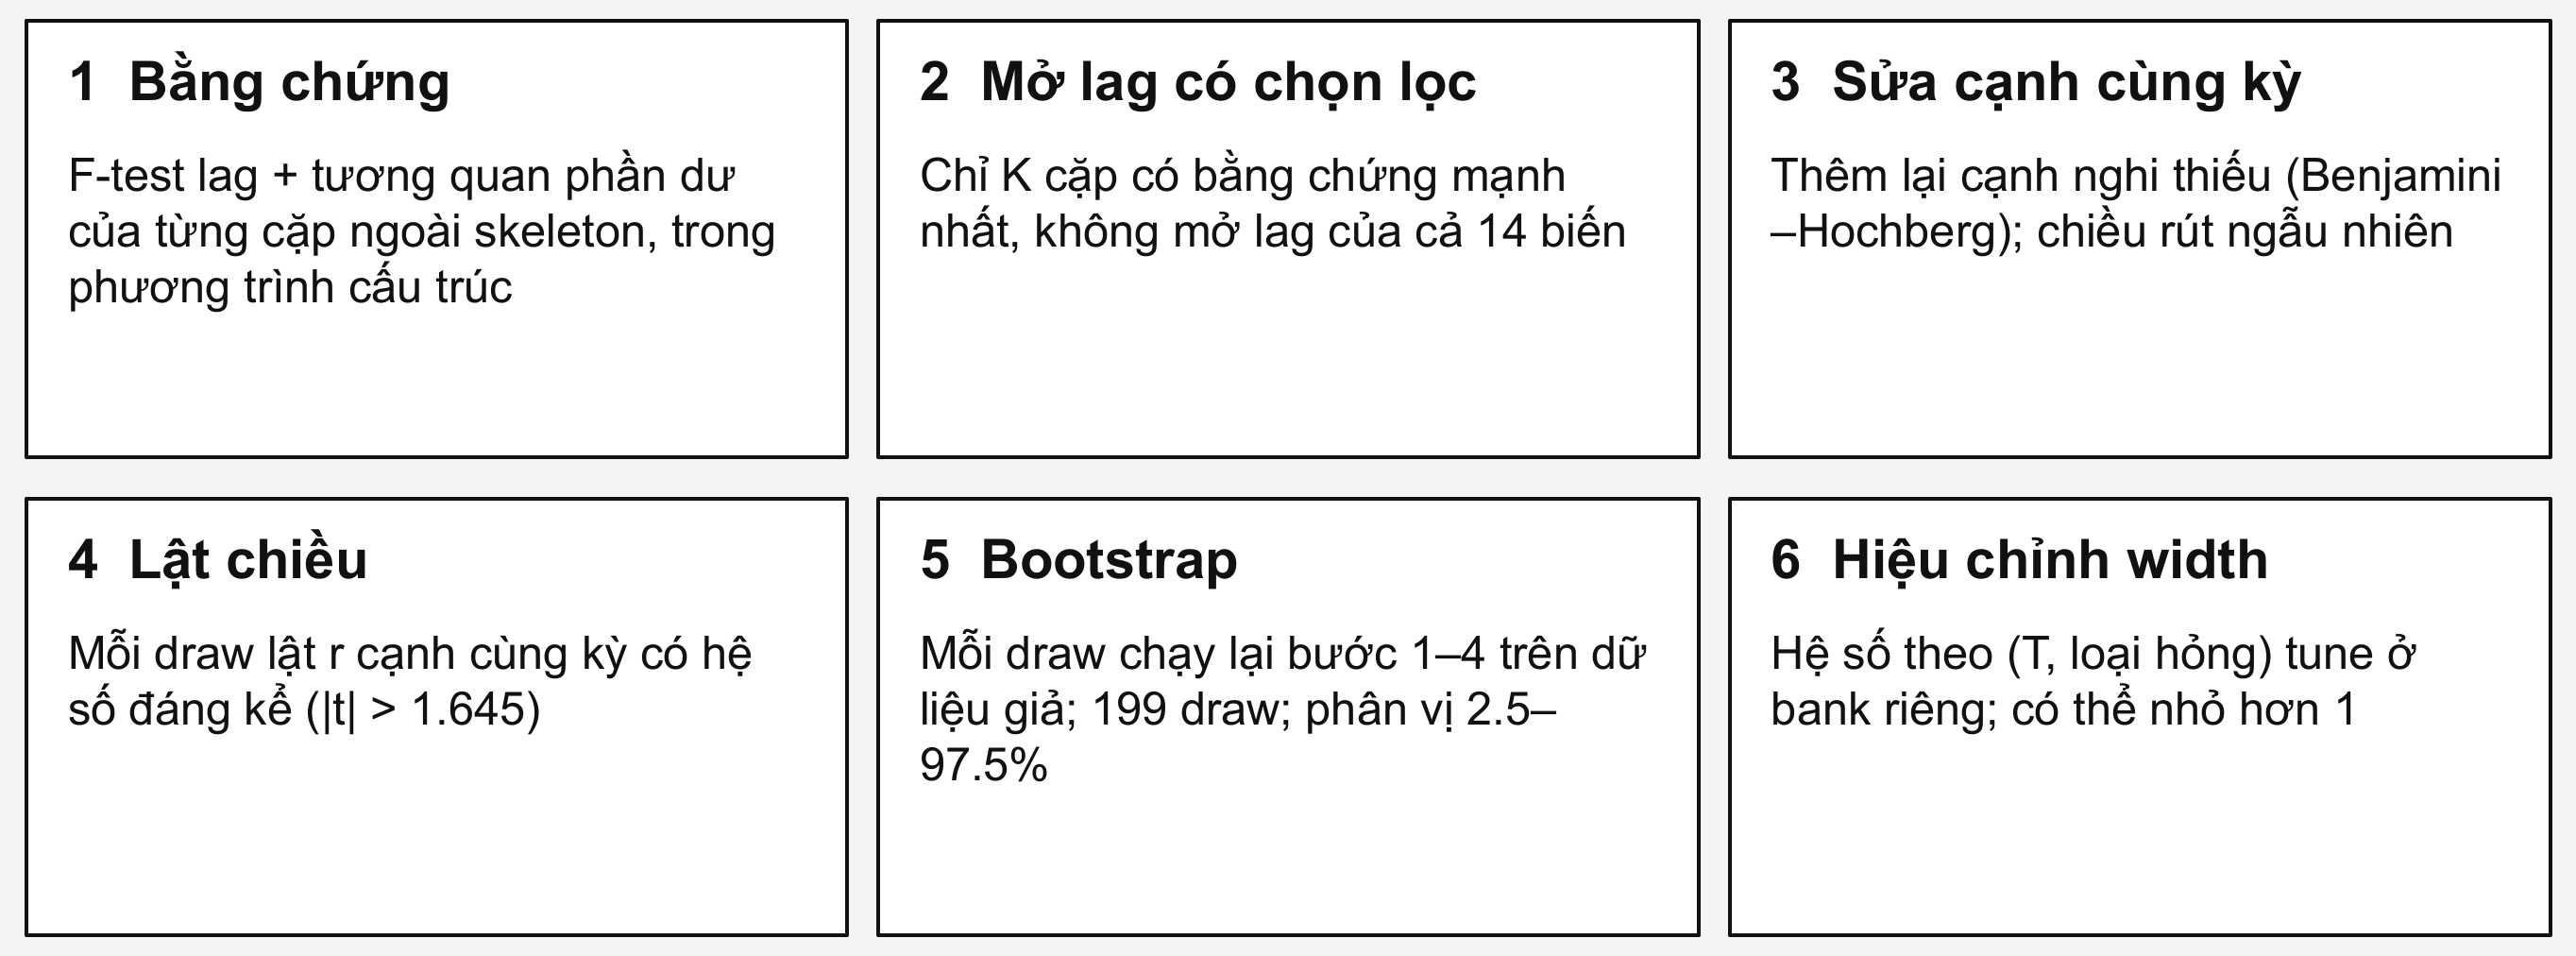
\includegraphics[width=\textwidth]{figures/buoc_phuong_phap_ours.png}
\caption{Sáu bước của \ours{}.}\label{fig:ours}
\end{figure}

Đầu vào gồm dữ liệu $X\in\mathbb R^{T\times n}$, skeleton $\mathcal S$ (với tập cạnh cùng kỳ có hướng $\mathcal O$) và khai báo $(k_{\text{miss}},k_{\text{extra}},k_{\text{rev}})$. Gọi $\mathcal N$ là tập các cặp \emph{không nối} trong $\mathcal S$. Đầu ra là $\hat C_{ji}(H)$ và $[\ell_{ji},u_{ji}]$ cho mọi cặp có thứ tự.

\subsection{Bước 1: chấm bằng chứng cho từng cặp không nối}
Với mỗi cặp $\{u,v\}\in\mathcal N$, chúng tôi chạy ba kiểm định \emph{trong phương trình cấu trúc của skeleton} (lag của chính nút, lag của các cặp nối, các cha cùng kỳ của skeleton):
\begin{enumerate}
  \item F-test thêm khối lag của $u$ vào phương trình của $v$;
  \item F-test thêm khối lag của $v$ vào phương trình của $u$;
  \item Fisher $z$ trên tương quan giữa phần dư cấu trúc của $u$ và của $v$ (dấu vết của một cạnh cùng kỳ bị thiếu).
\end{enumerate}
Ba $p$-value $p_1,p_2,p_3$ được gộp bằng phép hiệu chỉnh Šidák \citep{sidak1967rectangular}:
\begin{equation}
p_{uv}=1-\bigl(1-\min(p_1,p_2,p_3)\bigr)^3.
\end{equation}
Phân phối F được xấp xỉ bằng xấp xỉ chuẩn của Paulson. Kiểm định được đặt trong phương trình cấu trúc thay vì trong reduced-form VAR, vì ở reduced-form hiệu ứng truyền qua cạnh cùng kỳ làm các cặp không nối nhau trông như có quan hệ Granger, nên test không còn là test về sự kề nhau.

\subsection{Bước 2: mở khối lag có chọn lọc (targeted lag opening)}
Sắp xếp các cặp theo $p_{uv}$ tăng dần và mở khối lag (cả hai chiều) cho $K$ cặp đầu:
\begin{equation}
K=\min\Bigl(|\mathcal N|,\ \max\bigl(\lceil 3k_{\text{miss}}\rceil,\ \#\{p_{uv}<0.10\}\bigr)\Bigr).
\end{equation}
Số cạnh thiếu khai báo đặt \emph{sàn} cho lượng được mở ($3k_{\text{miss}}$); bằng chứng mạnh có thể mở nhiều hơn.

\subsection{Bước 3: bổ sung cạnh cùng kỳ (contemporaneous repair)}
Cạnh cùng kỳ bị thiếu để lại tương quan giữa các phần dư cấu trúc. Chúng tôi kiểm định các cặp không nối bằng thủ tục Benjamini--Hochberg \citep{benjamini1995controlling} ở mức $q=0.1$ rồi thêm lại tối đa $k_{\text{miss}}$ cạnh, mạnh nhất trước. Dữ liệu không xác định chiều của các cạnh này, nên mỗi lần chạy bootstrap rút chiều ngẫu nhiên; nếu chiều rút tạo chu trình thì lấy chiều còn lại.

\subsection{Bước 4: đảo chiều có chọn lọc (targeted reversal)}
Khi $k_{\text{rev}}>0$, mỗi lần chạy bootstrap lật $k_{\text{rev}}$ cạnh cùng kỳ, chọn trong các cạnh có hệ số cùng kỳ đáng kể ($|t|>1.645$ ở lần fit đầu) và không tạo chu trình.

\subsection{Bước 5: bootstrap có chọn lại cấu trúc}
Mỗi lần chạy bootstrap sinh dữ liệu giả $X^*$ từ phần dư (mục~\ref{sec:bootstrap}), rồi \emph{làm lại các bước 1--4 trên $X^*$} (chọn lại $K$ cặp, bổ sung cạnh, đảo chiều) và fit để được $\hat C^*(H)$. Với $B=199$ lần chạy, khoảng tin cậy là phân vị $2.5\%$--$97.5\%$ và điểm ước lượng là trung bình của các lần. Vì cấu trúc được chọn lại trong từng lần, khoảng tin cậy phản ánh nhiễu dữ liệu và bất định về cấu trúc, tức khoảng hiệu ứng trên các skeleton khả dĩ quanh skeleton đã cho.

\subsection{Bước 6: hiệu chỉnh độ rộng hai phía}
Khoảng từ bước 5 được co về trung điểm với hệ số $0.5$, rồi nhân với hệ số $c(T,\text{loại lỗi})$ chọn trên một tập dữ liệu hiệu chỉnh riêng, không dùng để chấm điểm, bằng lưới $1.0$--$10$ bước $0.1$. Hệ số hiệu dụng $0.5$--$5$ có thể nhỏ hơn 1, nên bước này nới được khoảng khi under-cover và thu hẹp được khi over-cover. Ví dụ khi thiếu cạnh, hệ số hiệu dụng là $1.3$ ở $T=80$ và $1.15$ ở $T=150$. Các hệ số được cố định trước và không chỉnh lại trên dữ liệu kiểm chứng; loại lỗi dùng để chọn hệ số là thành phần khai báo lớn nhất.

\begin{algorithm}[H]
\caption{\ours{}}
\begin{algorithmic}[1]
\Require $X$, skeleton $\mathcal S$, khai báo $(k_{\text{miss}},k_{\text{rev}})$, $B=199$
\State $\mathrm{Select}(X)\gets$ bước 1--3: tính $p_{uv}$, mở $K$ cặp, chọn ứng viên bổ sung cạnh
\State fit trên $X$ với skeleton, các cặp được mở và một lần rút cạnh bổ sung; thu $\hat B$ và phần dư $\hat u$
\For{$b=1,\dots,B$}
  \State $X^*\gets$ dựng chuỗi giả từ $\hat B$ và phần dư rút có hoàn lại
  \State $(\text{cặp mở}^*,\text{cạnh bổ sung}^*)\gets \mathrm{Select}(X^*)$ \Comment{chọn lại cấu trúc}
  \State rút chiều cho cạnh bổ sung; lật $k_{\text{rev}}$ cạnh (bước 4)
  \State fit trên $X^*$, tính $\hat C^{*(b)}(H)$ bằng \eqref{eq:irf}--\eqref{eq:cumulative}
\EndFor
\State $[\ell,u]\gets$ phân vị $2.5\%$, $97.5\%$ của $\{\hat C^{*(b)}\}$
\State co về trung điểm với hệ số $0.5$, rồi nhân $c(T,\text{loại lỗi})$ đã cố định
\State \Return $\hat C=\overline{\hat C^{*(b)}}$ và $[\ell,u]$
\end{algorithmic}
\end{algorithm}

\subsection{Trường hợp đặc biệt}
Khi không khai báo cạnh thiếu ($k_{\text{miss}}=0$), các bước 2--3 không chạy; phương pháp chỉ đảo chiều có chọn lọc rồi hiệu chỉnh độ rộng ở bước 6. Mỗi lần gọi mất khoảng $1.3$--$1.4$ giây ở $T=80$--$150$ với $n=14$ (bảng~\ref{tab:budget}).

\section{Thiết lập thực nghiệm}\label{sec:thiet-lap}

\subsection{Quy trình thực nghiệm}
Hình~\ref{fig:pipeline} tóm tắt quy trình một lượt thực nghiệm. Phía trên là mô hình thật, chỉ bước chấm điểm được truy cập; phía dưới là những gì phương pháp được thấy: dữ liệu, skeleton đã làm hỏng và số cạnh hỏng khai báo.

\begin{figure}[H]
\centering
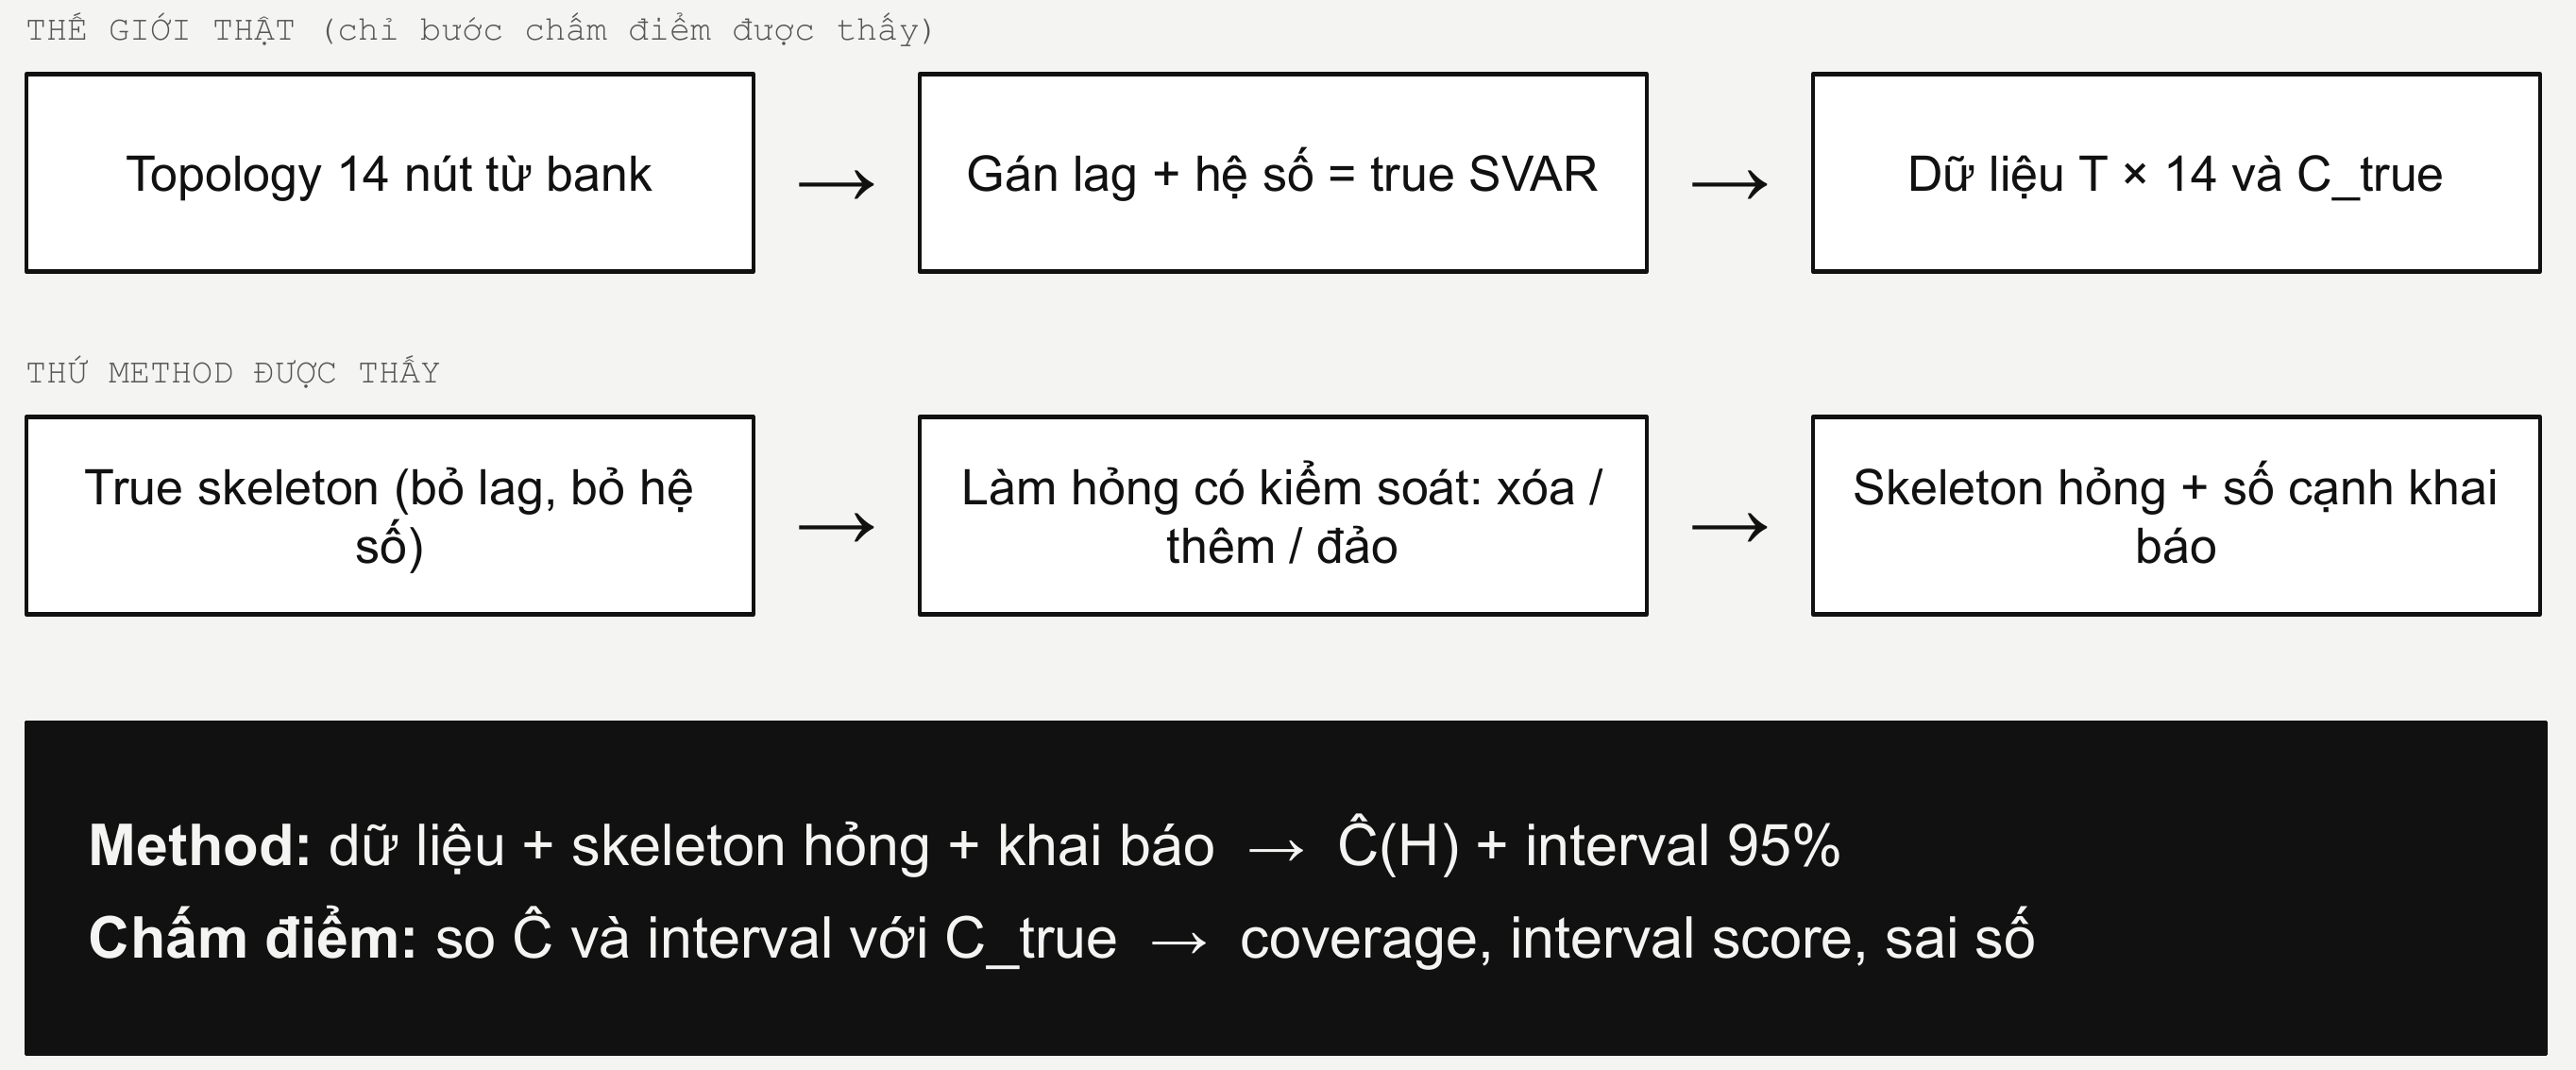
\includegraphics[width=\textwidth]{figures/quy_trinh_thuc_nghiem.png}
\caption{Quy trình một lượt thực nghiệm.}\label{fig:pipeline}
\end{figure}

Các bước cho mỗi bộ dữ liệu:
\begin{enumerate}
  \item Lấy một topology (đồ thị 14 nút, 21 cạnh).
  \item Gán lag và hệ số cho từng cạnh để được SVAR thật (mục~\ref{sec:generator}).
  \item Sinh $T\times14$ quan sát và tính $C(H)$ thật từ hệ số bằng \eqref{eq:irf}--\eqref{eq:cumulative}.
  \item Lấy skeleton thật (bỏ lag và hệ số), làm hỏng có kiểm soát (mục~\ref{sec:damage}) và ghi số cạnh hỏng làm khai báo.
  \item Đưa (dữ liệu, skeleton hỏng, khai báo) cho từng phương pháp; so $\hat C$ và khoảng tin cậy với $C(H)$ thật.
\end{enumerate}

\subsection{Sinh dữ liệu}\label{sec:generator}
Mỗi topology gồm 14 nút (7 ngân hàng, 3 biến vĩ mô, 4 chứng khoán) và 21 cạnh, thuộc hai họ đồ thị: Erdős--Rényi và scale-free có hub. Cấu trúc cạnh được sinh ngẫu nhiên.

\begin{table}[H]
\centering\small
\begin{tabularx}{\textwidth}{>{\raggedright\arraybackslash}p{4.3cm}Y}
\toprule
Thành phần & Cách rút\\
\midrule
Lag của mỗi cạnh & Cùng kỳ (lag 0) với xác suất $0.3$; còn lại ngẫu nhiên trong $\{1,\dots,p\}$, mặc định $p=2$ (khảo sát vùng dùng được thử $p\in\{1,2,4\}$)\\
Hệ số cạnh & $|b|\sim U(0.3,0.8)$, dấu ngẫu nhiên\\
Tự hồi quy & Hệ số lag 1 của mỗi nút $\sim U(0.2,0.6)$\\
Phương sai nhiễu & $\sigma_j^2\sim U(0.5,1.5)$ cho mỗi nút\\
Ổn định & Co phần lag đến khi bán kính phổ của ma trận companion $<0.9$\\
Burn-in & 200 quan sát đầu bị bỏ\\
Cỡ mẫu & $T\in\{40,80,150\}$ trong thực nghiệm chính; $T$ nhỏ tới $19$ trong khảo sát vùng dùng được\\
\bottomrule
\end{tabularx}
\caption{Tham số của bộ sinh dữ liệu.}
\end{table}

\subsection{Làm hỏng skeleton}\label{sec:damage}
Số cặp bị hỏng là $k=\lfloor \text{tỷ lệ}\times\text{cơ sở}+0.5\rfloor$, với cơ sở là số cạnh thật (21), hoặc, với đảo chiều, số cạnh cùng kỳ có thể đảo. Với 21 cạnh, tỷ lệ 20\% cho $k=4$ và 50\% cho $k=11$. Mỗi loại lỗi (thiếu, thừa, đảo) được thử ở hai mức 20\% và 50\%, cộng với trường hợp không hỏng: tổng cộng 7 cell. Phương pháp chỉ nhận cặp nối, chiều cạnh cùng kỳ và khai báo; không nhận danh sách cạnh hỏng, lag, hệ số hay $C(H)$ thật.

\subsection{Quy mô thực nghiệm}\label{sec:quymo}
Với mỗi cell, chúng tôi dùng một tập gồm 20 topology, mỗi topology 3 lần sinh dữ liệu độc lập, tổng cộng 60 bộ dữ liệu. Trên mỗi bộ dữ liệu, mỗi phương pháp chạy residual bootstrap $B=199$ lần để dựng khoảng tin cậy 95\% (phân vị 2.5\%--97.5\%). Thực nghiệm chính gồm 3 giá trị $T$, 7 cell và 60 bộ dữ liệu, tức $1260$ bộ cho mỗi phương pháp và khoảng $250$ nghìn lần fit.

Mỗi bộ có khoảng 30--40 cặp non-null, nên coverage của một cell được tính trên khoảng 2000 phép kiểm. Cặp mà phương pháp làm mất đường truyền ($\hat C=0$, khoảng $[0,0]$) được tính là trượt.

\subsection{Dữ liệu phát triển, hiệu chỉnh và kiểm chứng}
Chúng tôi dùng ba loại tập dữ liệu, mỗi loại gồm các topology khác nhau:
\begin{itemize}
  \item \textbf{Tập phát triển:} nơi thiết kế và thử phương pháp. Kết quả trên tập này mang tính thăm dò (exploratory) vì phương pháp có thể bị chỉnh theo chính nó.
  \item \textbf{Tập hiệu chỉnh:} chỉ dùng để chọn hệ số độ rộng (bước 6); không dùng để chấm điểm.
  \item \textbf{Tập kiểm chứng:} các tập topology sinh riêng bằng seed khác, chưa từng được dùng khi thiết kế phương pháp, không trùng cạnh với tập nào trước. Quy tắc kết luận được ghi trước khi chạy cùng giá trị băm (sha256) của code và cấu hình, và mỗi tập kiểm chứng chỉ được dùng một lần cho mỗi nhóm kết luận.
\end{itemize}
Các kết quả trong mục~\ref{sec:ket-qua} được gắn nhãn \emph{kiểm chứng} hoặc \emph{thăm dò} theo đúng nguồn dữ liệu này.

\subsection{Các phương pháp tham chiếu}\label{sec:baseline}
Bảng~\ref{tab:baselines} liệt kê các phương pháp tham chiếu cùng tên gọi trong tài liệu gốc. Phần sau mô tả từng phương pháp theo công trình gốc và cách áp dụng vào bài toán SVAR có skeleton cho sẵn. Hậu tố ``(cal)'' nghĩa là khoảng được nhân thêm hệ số độ rộng chọn theo $(T,\text{loại lỗi khai báo})$ trên tập hiệu chỉnh, theo đúng cách áp dụng cho \ours{}.

\begin{table}[H]
\centering\small
\begin{tabularx}{\textwidth}{>{\raggedright\arraybackslash}p{2.9cm}>{\raggedright\arraybackslash}p{4.3cm}Y}
\toprule
Ký hiệu & Tên trong công trình gốc & Nguồn\\
\midrule
Residual Bootstrap (RB) & Residual bootstrap cho IRF của VAR & \citet{kilian1998small}; \citet{efron1979bootstrap}\\
Oracle & RB trên đồ thị và lag thật & (mốc tham chiếu)\\
Inflate & Khoảng RB nới theo hệ số cố định & ---\\
Bagging & Bootstrap aggregation (bagging) & \citet{breiman1996bagging}\\
LP & Local projection; lag-augmented local projection & \citet{jorda2005estimation}; \citet{montiel2021local}\\
IDA & IDA (Intervention calculus when the DAG is Absent) & \citet{maathuis2009estimating}\\
BVAR-Minnesota & Bayesian VAR với Minnesota prior; chọn hyperparameter bằng marginal likelihood & \citet{doan1984forecasting}; \citet{litterman1986forecasting}; \citet{giannone2015prior}\\
PSel-Union & Post-selection inference for causal effects after causal discovery & \citet{chang2026post}\\
TLP & Targeted Local Projections; double bootstrap & \citet{nemtyrev2026targeted}\\
Full VAR & Unrestricted VAR & \citet{sims1980macroeconomics}\\
\bottomrule
\end{tabularx}
\caption{Các phương pháp tham chiếu và tên gọi trong tài liệu gốc.}\label{tab:baselines}
\end{table}

\paragraph{Residual Bootstrap và Oracle.}
Ước lượng SVAR đệ quy bằng OLS từng phương trình rồi dựng khoảng tin cậy cho IRF bằng cách rút phần dư có hoàn lại và fit lại \citep{kilian1998small,lutkepohl2005new,kilian2017structural}. Chúng tôi cắm skeleton vào mô hình \eqref{eq:svar}, chạy bootstrap $B=199$ lần và lấy phân vị 2.5\%--97.5\% (mục~\ref{sec:bootstrap}). Skeleton được giữ nguyên ở mọi lần chạy. Oracle là cùng quy trình trên đồ thị thật với lag đúng.

\paragraph{Inflate.}
Khoảng của RB được nới quanh trung điểm bởi hằng số $c$: $[m-c\,h,\;m+c\,h]$, với $m$ là trung điểm và $h$ là nửa độ rộng. $c$ được chọn theo từng $T$ trên tập hiệu chỉnh.

\paragraph{Bagging \citep{breiman1996bagging}.}
Bagging huấn luyện nhiều bản của một ước lượng trên các mẫu bootstrap rồi lấy trung bình để giảm phương sai. Ở đây mỗi lần chạy, skeleton bị xáo trộn ngẫu nhiên theo đúng loại và mức khai báo (thiếu: thêm $k$ cặp chưa có chiều với hạng tử lag; thừa: bỏ $k$ cặp; đảo: lật $k$ cạnh cùng kỳ mà không tạo chu trình), fit trên một mẫu bootstrap, và khoảng tin cậy là phân vị của các lần chạy.

\paragraph{LP: local projection \citep{jorda2005estimation,montiel2021local}.}
Local projection ước lượng $C_{ji}(H)$ bằng hồi quy trực tiếp $\sum_{h\le H}x_{j,t+h}$ lên $x_{i,t}$ và các biến điều khiển, không cần mô hình động đầy đủ. \citet{montiel2021local} chỉ ra rằng thêm một lag phụ vào biến điều khiển cho phép suy luận HAC thông thường mà không cần biết mức độ bền (persistence) của chuỗi. Ở đây hồi quy dùng $x_{i,t}$, các cha cùng kỳ của $i$ trong skeleton và lag $1..p{+}1$ của mọi nút, với sai số chuẩn Newey--West.

\paragraph{IDA \citep{maathuis2009estimating}.}
Khi đồ thị chỉ được biết đến lớp tương đương Markov (CPDAG), hiệu ứng nhân quả không xác định duy nhất. IDA ước lượng hiệu ứng theo từng đồ thị khả dĩ trong lớp rồi báo tập các giá trị. Ở đây chiều của skeleton chỉ được tin đến lớp tương đương; mỗi thành viên của lớp (tối đa 16) được fit như RB, khoảng tin cậy là union các khoảng và điểm ước lượng là trung bình.

\paragraph{BVAR-Minnesota \citep{doan1984forecasting,litterman1986forecasting,giannone2015prior}.}
Minnesota prior co hệ số của VAR về 0 với độ siết tăng theo lag; \citet{giannone2015prior} chọn hyperparameter bằng marginal likelihood. Ở đây mỗi phương trình có lag $1..p$ của mọi nút và các cha cùng kỳ của skeleton. Phương sai prior của hệ số lag $l$ của $x_i$ trong phương trình của $x_j$ là $(\lambda/l)^2\,s_j^2/s_i^2$, nhân thêm $\theta$ khi $i\ne j$ và cặp nằm ngoài skeleton, trong đó $s_i$ là độ lệch chuẩn phần dư của AR$(p)$ đơn biến. $(\lambda,\theta)$ được chọn trên lưới bằng marginal likelihood và khoảng tin cậy lấy từ các mẫu posterior.

\paragraph{PSel-Union \citep{chang2026post}.}
Công trình gốc xét suy luận nhân quả sau khi khám phá đồ thị: chạy thuật toán PC nhiều lần với test statistic bị thêm nhiễu ngẫu nhiên, giữ các đồ thị thu được và lấy union khoảng tin cậy; coverage đúng theo tiệm cận. Phương pháp gốc làm việc trên dữ liệu i.i.d. Gaussian, không có lag. Ở đây bước chọn được áp dụng trên VAR:
\begin{enumerate}
  \item Mỗi cặp được chọn khi z-score Granger (hai chiều) hoặc z-score tương quan riêng của phần dư vượt $1.96$. Mỗi lần chọn cộng nhiễu $\mathcal N(0,\tau^2)$ vào mọi z-score; lặp 100 lần.
  \item Giữ đồ thị không nhiễu và các đồ thị nhiễu xuất hiện nhiều nhất, tối đa $16$.
  \item Cặp được chọn mà skeleton chưa có chiều được fit theo cả hai chiều với hạng tử cùng kỳ.
  \item Mỗi thành viên chạy đủ $199$ lần bootstrap; khoảng tin cậy là union (min của cận dưới, max của cận trên) qua mọi thành viên.
\end{enumerate}
Phương pháp không đọc mức hỏng khai báo. Mỗi lần gọi dùng khoảng $6368$ lần bootstrap, gấp $32$ lần \ours{}. Chúng tôi báo cáo bản có và không có hiệu chỉnh độ rộng (PSel-Union, PSel-Union (cal)) cùng một biến thể rút gọn với tối đa $16$ đồ thị và ít lần bootstrap hơn (PSel).

\paragraph{TLP: Targeted Local Projections \citep{nemtyrev2026targeted}.}
TLP co ước lượng LP về một mô hình có cấu trúc (VAR) làm mục tiêu, theo trọng số tối ưu MSE:
\begin{equation}
\hat\beta^{\mathrm{TLP}}_h=v_h\,\hat\beta^{\mathrm{LP}}_h+(1-v_h)\,\hat\beta^{\mathrm{VAR}}_h,\qquad
v_h=\max\Bigl[1-\frac{\Sigma^{\mathrm{LP}}_h-\Sigma^{\mathrm{COV}}_h}{T(\hat\beta^{\mathrm{LP}}_h-\hat\beta^{\mathrm{VAR}}_h)^2},\,0\Bigr].
\end{equation}
Suy luận dùng double bootstrap hai tầng: tầng một bootstrap phần dư của VAR rút gọn, tầng hai lặp lại thủ tục trên từng mẫu của tầng một. Ở đây mô hình mục tiêu là RB trên skeleton cho sẵn, nên các ràng buộc zero của skeleton đóng vai sai lệch cục bộ khi skeleton hỏng. TLP (cal) dùng bootstrap một tầng kiểu VAR-sieve; TLP-DB dùng double bootstrap với số lag LP $p=3$ và $200\times100$ lần bootstrap.

\paragraph{Full VAR \citep{sims1980macroeconomics}.}
VAR không ràng buộc với lag của mọi nút trong mọi phương trình, cộng các cạnh cùng kỳ của skeleton; không bổ sung cạnh, không chọn lọc lag. Đây là cách mở mọi lag mà \ours{} tránh.

\subsection{Chi phí tính toán}
Bảng~\ref{tab:budget} so sánh số lần bootstrap và thời gian mỗi lần gọi. PSel-Union (cal), phương pháp tham chiếu mạnh nhất, dùng gấp $32$ lần số lần bootstrap và $6.6$--$7.9$ lần thời gian của \ours{}.
\begin{table}[H]
\centering\small
\begin{tabularx}{\textwidth}{lYrr}
\toprule
Phương pháp & Số lần bootstrap mỗi lần gọi & s/gọi, $T{=}80$ & $T{=}150$\\
\midrule
\ours{} & 199 (chọn lại lag mỗi lần) & 1.27 & 1.44\\
PSel-Union (cal) & 16 đồ thị, 32 thành viên $\times$ 199, trung bình 6368 & 8.34 & 11.42\\
PSel & $\le16$ đồ thị $\times\max(10,199\!\div\!\#)$ & 0.28 & 0.36\\
Full VAR (cal) & 199 & 0.51 & 0.61\\
TLP (cal) & 199 (VAR-sieve một tầng) & 0.31 & 0.40\\
TLP-DB & $200\times100$ & 5.14 & 6.03\\
BVAR-Minnesota (cal) & 199 mẫu posterior & 0.09 & 0.08\\
\bottomrule
\end{tabularx}
\caption{Chi phí tính toán (median của 6 lần gọi trên tập phát triển).}\label{tab:budget}
\end{table}

\subsection{Chỉ số đánh giá}\label{sec:metric}
\begin{description}
  \item[Coverage] tỷ lệ khoảng tin cậy chứa giá trị thật; mục tiêu khoảng $0.95$.
  \item[Độ rộng] $u-\ell$. Hẹp chỉ có ý nghĩa khi coverage đạt.
  \item[Interval score (IS)] \citep{gneiting2007strictly}. Với khoảng $[\ell,u]$ mức $1-\alpha$ và giá trị thật $c$:
  \begin{equation}
  \IS_\alpha(\ell,u;c)=(u-\ell)+\frac{2}{\alpha}(\ell-c)\,\mathbf 1\{c<\ell\}+\frac{2}{\alpha}(c-u)\,\mathbf 1\{c>u\}.
  \end{equation}
  Với $\alpha=0.05$, hệ số phạt là $2/\alpha=40$. IS càng thấp càng tốt và gộp cả độ rộng lẫn việc trượt. Ví dụ với $c=1.0$: khoảng $[0.8,1.2]$ có $\IS=0.4$; khoảng $[1.1,1.2]$ trượt $0.1$ có $\IS=0.1+40\times0.1=4.1$; khoảng $[-5,7]$ chứa $c$ nhưng quá rộng có $\IS=12$. IS của một lượt chạy là trung bình trên các cặp non-null.
  \item[Sai số cường độ] $|\hat C-C|$, tuyệt đối và tương đối.
  \item[Sai số lag] lệch mean lag và việc peak lag có đúng không.
\end{description}

\subsection{Phương pháp thống kê}
So sánh giữa hai phương pháp dùng hiệu IS trên cùng bộ dữ liệu. Vì các bộ dữ liệu cùng topology không độc lập, khoảng tin cậy 95\% của hiệu được tính bằng cluster bootstrap, resample cả topology; một cell chỉ được tính khi có ít nhất 8 cụm topology. Các so sánh trong cùng một họ được hiệu chỉnh đa kiểm định bằng phương pháp Holm \citep{holm1979simple} ở mức 0.05.

\section{Kết quả}\label{sec:ket-qua}

Các kết quả được gắn nhãn theo nguồn dữ liệu (mục~\ref{sec:thiet-lap}): \emph{kiểm chứng} nghĩa là đo trên tập topology chưa dùng khi thiết kế phương pháp, với quy tắc ghi trước; \emph{thăm dò} nghĩa là đo trên tập phát triển.

\subsection{Residual Bootstrap khi skeleton có lỗi (kiểm chứng)}\label{sec:rb}
Bảng~\ref{tab:full} so sánh RB (cắm skeleton như đúng) với \ours{} ở mọi loại lỗi và mọi cỡ mẫu, mỗi ô là coverage / interval score trên 60 bộ dữ liệu.

\begin{table}[H]
\centering\footnotesize
\setlength{\tabcolsep}{3pt}
\begin{tabular}{lcccccc}
\toprule
 & \multicolumn{2}{c}{$T=40$} & \multicolumn{2}{c}{$T=80$} & \multicolumn{2}{c}{$T=150$}\\
\cmidrule(lr){2-3}\cmidrule(lr){4-5}\cmidrule(lr){6-7}
Loại và mức lỗi & RB & \ours{} & RB & \ours{} & RB & \ours{}\\
\midrule
Không hỏng & 0.86 / 4.5 & 0.92 / 4.24 & 0.88 / 2.6 & 0.95 / 2.37 & 0.91 / 1.6 & 0.96 / 1.56 \\
Thừa 20\% & 0.87 / 4.5 & 0.93 / 4.33 & 0.88 / 2.7 & 0.93 / 2.51 & 0.92 / 1.6 & 0.96 / 1.59 \\
Thừa 50\% & 0.87 / 4.8 & 0.94 / 4.52 & 0.89 / 2.8 & 0.94 / 2.52 & 0.91 / 1.7 & 0.96 / 1.62 \\
Thiếu 20\% & 0.68 / 11.0 & 0.93 / 4.62 & 0.66 / 10.7 & 0.96 / 2.68 & 0.67 / 10.5 & 0.96 / 1.75 \\
Thiếu 50\% & 0.34 / 28.3 & 0.95 / 4.99 & 0.33 / 28.9 & 0.97 / 2.89 & 0.33 / 29.3 & 0.96 / 1.99 \\
Đảo 20\% & 0.84 / 5.1 & 0.94 / 4.52 & 0.83 / 3.9 & 0.95 / 2.73 & 0.83 / 2.9 & 0.95 / 1.84 \\
Đảo 50\% & 0.77 / 6.7 & 0.92 / 5.02 & 0.74 / 5.4 & 0.94 / 2.91 & 0.72 / 5.4 & 0.94 / 2.00 \\
Skeleton do GES$^{\dagger}$ & 0.38 / 22.8 & 0.98 / 9.19 & 0.34 / 23.0 & 0.95 / 3.58 & 0.32 / 21.7 & 0.93 / 2.74 \\
\bottomrule
\end{tabular}
\caption{Coverage / interval score của RB và \ours{}. $^{\dagger}$Skeleton học bằng GES từ chính dữ liệu; khai báo là mức lỗi GES trung bình đo trên tập hiệu chỉnh, và cột \ours{} của dòng này là phiên bản trước chọn lọc lag (chưa chạy \ours{}).}\label{tab:full}
\end{table}

Ba nhận xét:
\begin{itemize}
  \item \textbf{RB hỏng nặng nhất khi thiếu cạnh và với skeleton do GES học ra.} Khi thiếu 50\% cạnh, RB chỉ phủ khoảng $0.33$ với IS gần $29$; với skeleton do GES học ra, RB phủ $0.32$--$0.38$ với IS khoảng $22$. Cạnh đảo làm coverage giảm xuống $0.72$--$0.84$; cạnh thừa chỉ giảm nhẹ.
  \item \textbf{RB không đạt mức danh nghĩa ngay cả khi skeleton đúng:} coverage $0.86$, $0.88$, $0.91$ ở $T=40,80,150$. Một phần cải thiện của \ours{} là do hiệu chỉnh độ rộng, không phải do xử lý cấu trúc.
  \item \textbf{\ours{} giữ coverage trong khoảng $0.92$--$0.97$} ở mọi ô, nhưng chưa đạt $0.95$ ở một số ô (ví dụ $0.92$ ở $T=40$ khi không hỏng hoặc đảo 50\%). Cái giá so với skeleton đúng nhỏ: ở $T=80$, IS là $2.37$ khi không hỏng và $2.68$ khi thiếu 20\% cạnh.
\end{itemize}

\subsection{So sánh với các phương pháp tham chiếu khi thiếu cạnh (RQ4.2, kiểm chứng)}\label{sec:main}
Các phương pháp tham chiếu chỉ được chạy ở bốn cell thiếu cạnh với $T\in\{80,150\}$ và tỷ lệ cạnh thiếu 20\%, 50\% (60 bộ dữ liệu mỗi cell), nên so sánh dưới đây chỉ có giá trị trong phạm vi này. Bảng~\ref{tab:main} là interval score (coverage trong ngoặc); IS thấp hơn là tốt hơn.

\begin{table}[H]
\centering\small
\begin{tabular}{lcccc}
\toprule
Phương pháp & $T{=}80$, 20\% & $T{=}80$, 50\% & $T{=}150$, 20\% & $T{=}150$, 50\%\\
\midrule
RB & 10.68 (0.655) & 28.94 (0.335) & 10.54 (0.668) & 29.25 (0.325)\\
\textbf{\ours{}} & \textbf{2.68} (0.963) & \textbf{2.89} (0.969) & \textbf{1.75} (0.964) & \textbf{1.99} (0.960)\\
PSel-Union & 3.46 (0.968) & 3.41 (0.978) & 2.15 (0.983) & 2.30 (0.988)\\
PSel-Union (cal) & 3.30 (0.943) & 3.20 (0.952) & 1.95 (0.950) & 2.04 (0.959)\\
PSel (cal) & 3.91 (0.962) & 4.12 (0.943) & 2.62 (0.972) & 3.06 (0.937)\\
Full VAR (cal) & 3.41 (0.973) & 3.74 (0.953) & 2.62 (0.976) & 3.01 (0.953)\\
TLP (cal) & 3.50 (0.955) & 3.75 (0.940) & 2.22 (0.979) & 2.43 (0.962)\\
TLP-DB & 3.71 (0.872) & 4.83 (0.804) & 2.21 (0.905) & 2.88 (0.857)\\
BVAR-Minnesota (cal) & 4.64 (0.969) & 4.44 (0.969) & 3.72 (0.953) & 3.79 (0.957)\\
\bottomrule
\end{tabular}
\caption{Interval score (coverage), các cell thiếu cạnh, tập kiểm chứng.}\label{tab:main}
\end{table}

Bảng~\ref{tab:diff} là hiệu IS giữa \ours{} và từng phương pháp tham chiếu trên cùng bộ dữ liệu (âm nghĩa là \ours{} tốt hơn).

\begin{table}[H]
\centering\small
\begin{tabular}{lcccc}
\toprule
Phương pháp tham chiếu & $T{=}80$, 20\% & $T{=}80$, 50\% & $T{=}150$, 20\% & $T{=}150$, 50\%\\
\midrule
PSel-Union & $-0.78$ & $-0.51$ & $-0.41$ & $-0.30$\\
PSel-Union (cal) & $-0.61$ & $-0.30$ & $-0.20$ & $-0.05$ (hòa)\\
PSel (cal) & $-1.22$ & $-1.22$ & $-0.87$ & $-1.07$\\
Full VAR (cal) & $-0.72$ & $-0.85$ & $-0.87$ & $-1.02$\\
TLP (cal) & $-0.82$ & $-0.85$ & $-0.47$ & $-0.44$\\
TLP-DB & $-1.02$ & $-1.93$ & $-0.46$ & $-0.89$\\
BVAR-Minnesota (cal) & $-1.96$ & $-1.54$ & $-1.97$ & $-1.80$\\
\bottomrule
\end{tabular}
\caption{Hiệu interval score giữa \ours{} và phương pháp tham chiếu.}\label{tab:diff}
\end{table}

\ours{} thắng có ý nghĩa ở $27/28$ so sánh (khoảng tin cậy 95\% của hiệu không chứa 0, Holm trên 56 so sánh) và không thua so sánh nào. Trường hợp hòa duy nhất là PSel-Union (cal) ở $T=150$, thiếu 50\%: hiệu $-0.05$, khoảng $[-0.17,+0.04]$; phương pháp đó dùng gấp 32 lần số lần bootstrap. Coverage của \ours{} ở bốn cell là $0.96$--$0.97$, hơi trên mức danh nghĩa. Có ba điều cần lưu ý khi đọc kết quả này. Thứ nhất, mức chênh so với phương pháp tham chiếu gần nhất là $0.05$--$0.8$ trên mức IS $2$--$4$, tức khoảng $2$--$25\%$, nhỏ hơn nhiều so với khoảng cách với RB. Thứ hai, \ours{} nhận số cạnh thiếu khai báo $k_{\text{miss}}$ để quyết định số cặp được mở, trong khi PSel-Union, BVAR-Minnesota và TLP không dùng $k_{\text{miss}}$ khi chọn cấu trúc (chỉ hệ số độ rộng của bản (cal) biết loại lỗi), nên lợi thế gộp cả phương pháp và thông tin khai báo. Thứ ba, ở $T=40$ (kết quả thăm dò) BVAR-Minnesota (cal) hòa với \ours{} khi thiếu cạnh và có IS thấp hơn $0.6$--$0.9$ khi cạnh thừa, không hỏng hoặc đảo 20\%. Lợi thế thu hẹp khi $T$ tăng, vì khi dữ liệu nhiều thì việc mở mọi lag cũng không còn tốn kém.

So với phiên bản không chọn lọc lag (mở mọi lag và chỉ hiệu chỉnh một phía), ở $T=40$ thiếu 20\% cạnh IS giảm từ $7.81$ xuống $4.62$ (hiệu $-3.19$, khoảng $[-3.54,-2.87]$) và thiếu 50\% giảm từ $7.54$ xuống $4.99$ ($-2.55$, $[-2.76,-2.34]$), với coverage $0.928$ và $0.947$; ở 19 cell còn lại không cell nào tệ hơn có ý nghĩa.

\subsection{Đóng góp của từng thành phần (thăm dò)}
\begin{table}[H]
\centering\small
\begin{tabularx}{\textwidth}{>{\raggedright\arraybackslash}p{5.3cm}Y}
\toprule
Thành phần & Tác dụng đo được\\
\midrule
Bổ sung cạnh cùng kỳ và rút chiều ngẫu nhiên & Nguồn lợi thế so với chỉ mở mọi lag: Full VAR (cal) tệ hơn ở 19/21 cell sau Holm\\
Hiệu chỉnh độ rộng hai phía & Giảm IS $0.71$--$0.79$ ở $T=40$ khi thiếu cạnh; ở cell khác gần như không đổi\\
Mở lag có chọn lọc, chọn lại trong từng lần bootstrap & Giảm IS ở cả 6 cell thiếu cạnh ($-0.23$ đến $-2.93$), không làm tệ cell nào\\
\bottomrule
\end{tabularx}
\caption{Đóng góp của từng thành phần của \ours{} trên tập phát triển.}
\end{table}

\subsection{Tác động của loại và mức hỏng (RQ4.1)}\label{sec:rq41}
Chúng tôi đánh giá RQ4.1 bằng bốn tiêu chí, kiểm tra trên ba tập kiểm chứng độc lập (lần 1, 2, 3), mỗi tập gồm 20 topology mới:
\begin{description}
  \item[(a) Thứ tự mức nặng.] Với RB trên các cặp bị hỏng, sai số tương đối theo thứ tự thiếu $>$ đảo $>$ thừa ở ít nhất $5/6$ cell ($T\in\{40,80,150\}\times$ tỷ lệ $\{0.2,0.5\}$). Tiêu chí sửa (a$'$): thiếu $>$ đảo \emph{và} thiếu $>$ thừa ở $4/4$ cell $T\ge80$; $T=40$ chỉ để mô tả.
  \item[(b)] Coverage của RB khi thiếu 50\% cạnh thấp hơn $0.60$ ở cả ba giá trị $T$.
  \item[(c) \ours{} so với RB.] Giảm sai số ở $6/6$ cell thiếu cạnh. Coverage trên cặp bị hỏng $\ge0.90$ ở $4/4$ cell ($T\in\{80,150\}\times\{0.2,0.5\}$). Tiêu chí sửa (c2): với mỗi $T\in\{80,150\}$, gộp hai mức hỏng, cận dưới của khoảng tin cậy 95\% (cluster bootstrap) $\ge0.85$.
  \item[(d)] Lỗi mean-lag của RB không giảm quá 25\% khi $T$ tăng từ $40$ lên $150$ ở các cell thiếu và đảo.
\end{description}

\begin{table}[H]
\centering\small
\begin{tabularx}{\textwidth}{>{\raggedright\arraybackslash}p{1.4cm}>{\raggedright\arraybackslash}p{2.4cm}CCCCY}
\toprule
Lần & Quy tắc & (a) & (b) & (c) & (d) & Kết luận\\
\midrule
1 & Gốc & Trượt, $4/6$ & Đạt & Đạt & Đạt & Không đạt\\
2 & (a$'$) & Đạt $4/4$ & Đạt & Trượt, $3/4$ & Đạt & Không đạt\\
3 & (a$'$), (c2) & Đạt $4/4$ & Đạt & Đạt & Đạt & Đạt theo tiêu chí sửa\\
\bottomrule
\end{tabularx}
\caption{Ba lần kiểm chứng RQ4.1.}
\end{table}
\begin{itemize}
  \item \textbf{Lần 1:} tiêu chí (a) trượt vì hai cell $T=40$ không tách được cạnh đảo khỏi cạnh thừa (khoảng tin cậy của hiệu chứa 0). Coverage của RB khi thiếu 50\% là $0.349/0.336/0.315$ ở $T=40/80/150$.
  \item \textbf{Lần 2:} (a$'$) đạt $4/4$. (c) trượt ở một cell: coverage của \ours{} trên cặp bị hỏng ở $T=80$, thiếu 20\% là $0.899$, thiếu $0.001$ so với ngưỡng $0.90$ (khoảng $[0.872,0.926]$ chứa $0.90$); coverage trên mọi cặp non-null là $0.953$--$0.967$. Coverage của RB khi thiếu 50\% là $0.373/0.350/0.335$.
  \item \textbf{Lần 3:} (a$'$) và (b) đạt; (c2) đạt cho cả hai phiên bản: phiên bản không chọn lọc lag $0.956$ ($T=80$) và $0.957$ ($T=150$); \ours{} $0.929$ $[0.916,0.942]$ và $0.947$ $[0.936,0.957]$.
\end{itemize}
Các tiêu chí (a$'$) và (c2) được chọn sau khi đã thấy kết quả lần 1 và lần 2, nghĩa là quy tắc được sửa sau khi có dữ liệu; ngưỡng $0.85$ và cách gộp theo $T$ được khóa trước khi chạy lần 3. Theo quy tắc gốc, RQ4.1 không đạt ở lần 1, và thứ tự đầy đủ thiếu $>$ đảo $>$ thừa vẫn chỉ đạt $4/6$ ở lần 2 và lần 3. Phần kết luận định tính chắc chắn là: thiếu cạnh là loại lỗi nặng nhất, cạnh thừa gần như vô hại với cường độ, cạnh đảo làm sai cả lag; ở $T=40$ chưa tách được đảo khỏi thừa.

\subsection{Bản đồ chi phí theo cạnh (RQ4.3, kiểm chứng)}
Với mỗi cạnh của skeleton, chúng tôi đo hiệu ứng lệch bao nhiêu khi cạnh đó sai. Độ lệch trung vị của các cặp nằm \emph{trên đường truyền dẫn} của cạnh hỏng là: thiếu cạnh cùng kỳ $0.952$ $[0.929,0.965]$, thiếu cạnh có lag $0.844$ $[0.749,0.895]$, đảo cạnh cùng kỳ $0.541$ $[0.510,0.574]$. Bản đồ ổn định: hệ số tương quan Spearman giữa hai nửa topology là $0.993$ và giữa hai họ đồ thị (Erdős--Rényi và hub) là $0.965$; Holm đạt $12/12$.

\subsection{Cờ độ tin cậy (RQ4.4, kiểm chứng)}
Chúng tôi huấn luyện trước một mô hình logistic với ba đặc trưng quan sát được (độ rộng, độ rộng tương đối, mức hỏng khai báo) và không fit lại khi kiểm chứng. AUROC là $0.720$ $[0.698,0.744]$ ở $T=80/150$ và $0.812$ $[0.791,0.832]$ ở $T=40$, cao hơn comparator độ rộng tương đối $+0.089$ và $+0.220$. Cặp bị gắn cờ trượt nhiều gấp $3.98$ lần ($T=80/150$) và $6.77$ lần ($T=40$). Các diagnostic quen thuộc như độ ổn định hệ số hay phần dư không dự báo được theo chiều kỳ vọng.

\subsection{Vùng dùng được (thăm dò)}\label{sec:vung}
Một ô (số lag $p$, $T$, loại và mức hỏng) \emph{dùng được} với một phương pháp nếu: (i) ít nhất $57/60$ lượt chạy trả kết quả; (ii) coverage gộp $\ge0.90$; (iii) IS trung bình $\le3\times$ IS của Oracle ở cùng $(p,T)$, điều kiện này loại các khoảng ``phát nổ''. $T$ tối thiểu là $T$ nhỏ nhất sao cho mọi $T$ từ đó trở lên đều dùng được ở cả hai mức hỏng.
\begin{table}[H]
\centering\small
\begin{tabular}{ccc}
\toprule
$p$ & $T$ tối thiểu, \ours{} & $T$ tối thiểu, phiên bản không chọn lọc lag\\
\midrule
1 & 19 & 25\\
2 & 40 & 40\\
4 & 80 & 150\\
\bottomrule
\end{tabular}
\caption{$T$ tối thiểu khi thiếu cạnh.}\label{tab:vung}
\end{table}
Với $p=1$, một panel $14\times19$ nằm trong vùng dùng được của \ours{} ở các ô không hỏng, thiếu $0.2$ và $0.5$, đảo $0.2$; ô đảo $0.5$ thì không. Ở $T=19$, phiên bản không chọn lọc lag không chạy được lượt nào ($0/60$). Với $p=2$ và $T<40$, nhiều phương trình không ước lượng được, kể cả với RB, do số biến hồi quy vượt số dòng dữ liệu.

\subsection{Thảo luận}
\begin{itemize}
  \item \textbf{Thiếu cạnh là lỗi nặng nhất.} RB cho khoảng hẹp nhưng sai nên coverage chỉ $0.33$--$0.68$ khi thiếu cạnh; cạnh thừa gần như vô hại.
  \item \textbf{Mở mọi lag ở $T$ nhỏ làm khoảng phình rộng} ($28$ biến hồi quy trên $38$ dòng). \ours{} chỉ mở lag cho cặp có bằng chứng, nên IS thấp hơn rõ rệt ở $T=40$.
  \item \textbf{Khoảng của \ours{} rộng hơn RB} vì RB hẹp mà sai. Do đó RQ4.2 nên được phát biểu theo interval score, thước đo gộp độ rộng và việc trượt, thay vì chỉ theo độ rộng.
  \item \textbf{Lợi thế thu hẹp từ $T=150$:} phương pháp tham chiếu mạnh nhất hòa với \ours{} ở một cell.
\end{itemize}

\section{Kết luận}\label{sec:ket-luan}
Chúng tôi trình bày \ours{}, phương pháp ước lượng hiệu ứng tích lũy của SVAR khi skeleton có lỗi, dùng số cạnh hỏng khai báo để quyết định mở bao nhiêu khối lag, chọn lại cấu trúc trong từng lần bootstrap và hiệu chỉnh độ rộng hai phía. Cắm skeleton hỏng vào residual bootstrap làm coverage giảm xuống khoảng $0.33$ khi thiếu 50\% cạnh và $0.32$--$0.38$ khi skeleton do GES học ra; \ours{} đưa coverage về $0.92$--$0.97$ ở mọi loại lỗi. Ở các cell thiếu cạnh với $T\ge80$, \ours{} có interval score thấp hơn các phương pháp tham chiếu đã thử (hòa một cell), với biên độ chênh khiêm tốn và với lưu ý rằng \ours{} dùng thêm số cạnh thiếu khai báo. Thiếu cạnh là loại lỗi nặng nhất, bản đồ chi phí theo cạnh ổn định giữa các topology, và một cờ độ tin cậy đơn giản dự báo được cặp nào dễ trượt. Vùng dùng được kéo xuống tới $T=19$ khi $p=1$, đủ cho panel thật 14 biến.


\bibliographystyle{plainnat}
\bibliography{references}
\end{document}
